% 使用默认的 beamer 文档类
\documentclass{beamer}
%%%%%%%%%%%%%%%%%%%%%%%%%%%%%%%%%%%%%%%%
%%%%%% 演示文稿样式
% 支持中文
\usepackage{ctex}
% 适应中文, 首行缩进
\usepackage{indentfirst}
% 设置缩进 2 个字符
\setlength{\parindent}{2em}
% 字体修改支持
\usepackage{fontspec}
% 添加信息栏, 必须放在 usetheme 之前
% \useoutertheme{infolines}
% 规定 theme采用
\usetheme{Madrid}
% 规定颜色主题采用
\usecolortheme{default}
% 删去底部导航图标
% \setbeamertemplate{navigation symbols}{}
%%%%%%%%%%%%%%%%%%%%%%%%%%%%%%%%%%%%%%%%
%%%%%%浮动体样式
% 浮动体不越过section
\usepackage[section]{placeins}
% 设置列表缩进
\usepackage[shortlabels]{enumitem}
% 三线表宏包
\usepackage{booktabs}
% 设置表格的列格式
\usepackage{array}
% 插图
\usepackage{graphicx}
% 浮动体宏包 可禁用浮动效果
\usepackage{float}
% 支持 beamer 为图片编号
\setbeamertemplate{caption}[numbered]
%%%%%%%%%%%%%%%%%%%%%%%%%%%%%%%%%%%%%%%%
%%%%%%代码样式
% 代码样式
% 设置等宽的代码字体
\usepackage{url}
% 建议这个: (linux?)
% \setmonofont{IBM Plex Mono}
% win 用户请
\setmonofont{Courier New}
%%%%%%%%%%%%%%%%%%%%%%%%%%%%%%%%%%%%%%%%
% 自定义命令

%%%%%%%%%%%%%%%%%%%%%%%%%%%%%%%%%%%%%%%%
% 文档备注
% 第一部分实验总结报告
% 截止 2021-4-27 下午11:55
% 允许重新提交的次数: 无限制
% 指导:
% 每位同学对02-06共5次实验进行总结,形成PPT格式报告.
% 报告内容包括但不限于: 实验过程(简), 实验心得, 遇到的问题,
% 与理论课联系, 对实验设置的建议等等.
% PPT报告时间不超过10分钟.
% 所有同学都需要提交PPT,该评分计入总成绩.

%%%%%%%%%%%%%%%%%%%%%%%%%%%%%%%%%%%%%%%%
% 文档信息
\title{计算机网络实验2-6总结}
\author{chuan-325}
\institute[UCAS]{University of Chinese Academy of Sciences}

%%%%%%%%%%%%%%%%%%%%%%%%%%%%%%%%%%%%%%%%
\begin{document}
\section*{封面}
% 封面页
\begin{frame}
    \maketitle
\end{frame}

\begin{frame}{索引}
    \tableofcontents
\end{frame}
%%%%%%%%%%%%%%%%%%%%%%%%%%%%%%%%%%%%%%%%
%%%%%%实验 2
\section{实验 2: 流完成时间实验}
% 节标题
\begin{frame}
    \sectionpage
\end{frame}

% 实验过程
\begin{frame}{实验过程}{实验 2: 流完成时间实验}
    \begin{block}{主要内容}
        验证\textbf{带宽},\textbf{时延}和\textbf{流大小}
        对\textbf{流完成时间}的影响.
    \end{block}
    \begin{block}{实验流程}
        1. 修改 fct\_exp.py 脚本中的参数以改变带宽和时延;\\
        2. 在 h2 节点创建不同大小的文件, 在 h1 节点通过 wget
        获取文件;\\
        3. 整理数据, 选择对数坐标, 绘制成图.
    \end{block}
\end{frame}

% 实验结果展示
\begin{frame}{实验结果展示}{实验 2: 流完成时间实验}
    根据实验数据制作的图大致复现了原图:
    \begin{figure}[h]
        \centering % 居中显示
        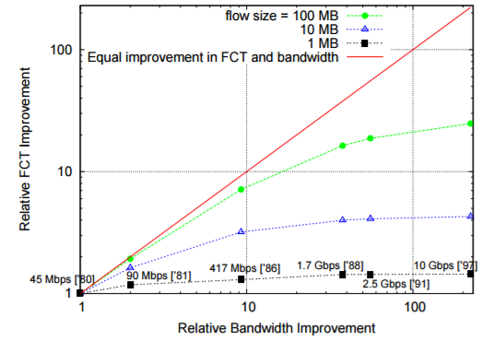
\includegraphics[scale=0.45]{figs/fct-paper.png}
        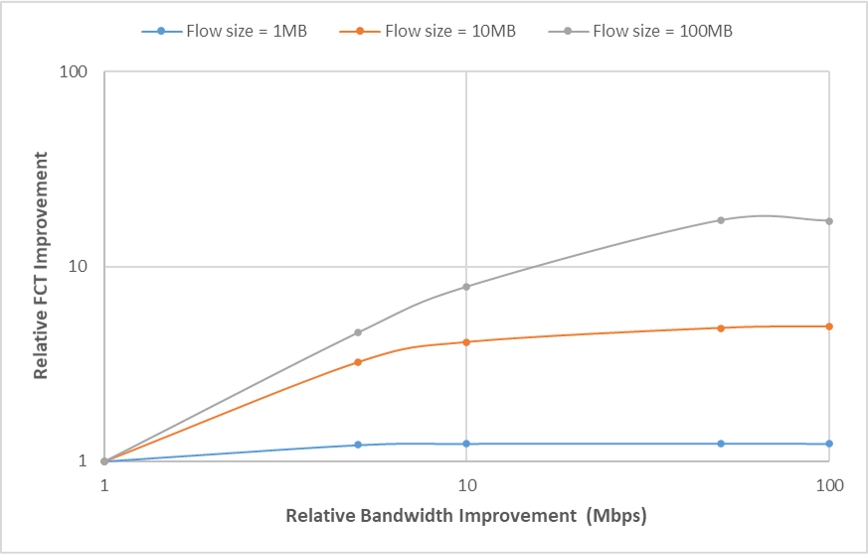
\includegraphics[scale=0.4]{figs/fct-improvement.png}
        \caption{原图(左) vs 根据实验数据制作的图 (右)} % 标题
    \end{figure}
\end{frame}

% 实验反思
\begin{frame}{实验反思}{实验 2: 流完成时间实验}
    \begin{block}{实验心得}
        1. 绘图时, 为了使实验效果更明显, 使用了对数坐标;\\
        2. 实验中, 手动执行测试效率太低, 可以使用脚本改变虚拟
        网络环境参数自动测试;\\
        3. 测试时, 一定要多次运行后求平均值.
    \end{block}

    % \begin{block}{遇到的问题}
    %     暂无.
    % \end{block}
\end{frame}

% 涉及的理论知识
\begin{frame}{涉及的理论知识}{实验 2: 流完成时间实验}
    实验内容涉及 TCP 传输中使用的拥塞控制方法.
    \newline\newline
    \begin{block}{慢启动算法 (slow-start)}
        每经过一个传输轮次, 就将拥塞窗口\textbf{加倍}.
    \end{block}

    慢启动算法既保证了传输的效率, 又避免了大量数据的
    突发性传输造成网络拥塞.
\end{frame}
\begin{frame}{涉及的理论知识}{实验 2: 流完成时间实验}
    在慢启动算法的基础上, 引入\textbf{慢开始门限} (ssthresh)
    概念, 得到对 TCP 传输全程均有调控拥塞避免算法:

    \begin{block}{拥塞避免算法 (congestion avoidance)}
        1. 在拥塞窗口到达慢开始门限之前, 每经过一个传输轮次
        就将拥塞窗口加倍;\\
        2. 以下情况之一发生后, 每经过 1 个往返时间,
        就将拥塞窗口+1:\\
        \quad 1. 拥塞窗口 (cwnd) 超过慢开始门限;\\
        \quad 2. 出现丢包;

        \quad 3. 到达接收方\textbf{接收窗口} (rwnd) 限制后.
    \end{block}

    拥塞避免算法在尽可能保证传输效率的同时, 减少了因 TCP 拥塞产生的丢包问题.
\end{frame}
\begin{frame}{TCP 拥塞控制对实验结果的影响}{实验 2: 流完成时间实验}
    \begin{block}{传输速率并非随着带宽增加线性增长}
        \textbf{原因:}
        慢开始机制规定了拥塞窗口在传输初期的增长机制,
        这使得文件传输的初始一段时间无法达到最大传输速度,
        并且这段时间相对于总传输时间无法忽略.
    \end{block}
    \begin{block}{小带宽情形下 FCT 相对难以提升}
        \textbf{原因:}
        小带宽情形下的慢开始门限较小, 达到门限也较快,
        故 FCT 始终被限制在相对较低的水平.
    \end{block}
\end{frame}
%%%%%%%%%%%%%%%%%%%%%%%%%%%%%%%%%%%%%%%%
%%%%%%实验 3
\section{实验 3: Socket编程实验}
% 节标题
\begin{frame}
    \sectionpage
\end{frame}

% 实验过程
\begin{frame}{实验过程}{实验 3: Socket编程实验}
    \begin{block}{主要内容}
        使用 C 语言实现最简单的 HTTP 服务器与 HTTP
        客户端, 且保证分别支持 HTTP GET 方法.
    \end{block}
    \begin{block}{实验流程}
        1. 编写完成 HTTP 服务器与 HTTP 客户端程序;\\
        2. 编译得到可执行文件, 使用 python 的 http
        服务器和 wget 分别替代服务器和客户端, 对客户端
        与服务器进行测试, 要求支持多次连续获取文件和
        多个客户端分别获取文件.
    \end{block}
\end{frame}
% 程序行为
\begin{frame}{程序行为}{实验 3: Socket编程实验}
    \begin{block}{HTTP 客户端}
        1. (socket) 在本地建立套接字, 成功则继续,
        否则报错退出;\\
        2. (connect) 主动建立到服务器的连接, 成功则继续,
        否则报错退出;\\
        3. (send) 对于用户输入的每一个文件URL,编码形成符合
        格式规范的 HTTP GET 请求, 并通过已建立的连接发送请求,
        若发送失败, 则报错退出;\\
        4. (recv) 接收来自服务器的 HTTP 应答报文, 解析报文,
        读取请求状态, 据此打印相关信息或存储文件;\\
        5. (while(1)) 一个请求接收完毕后, 等待用户的下一个输入,
        并据此决定是继续编码发送 HTTP 请求还是关闭连接和套接字退出程序.
    \end{block}
\end{frame}
\begin{frame}{程序行为}{实验 3: Socket编程实验}
    \begin{block}{HTTP 服务器}
        1. (socket, bind) 设置监听端口, 建立套接字,
        绑定监听端口并开始监听;\\
        2. (accept) 接收来自客户端的连接;\\
        3. 为了支持请求并发, 对于每一个成功建立的连接,
        都新建一个用来处理 HTTP 请求的 receiver 线程;\\
        4. (recv) 线程接收请求后, 根据接收长度判断是否有效请求;
        请求有效则解析得到文件名, 根据文件存在情况编码
        HTTP 应答报文;\\
        5. (send) 向客户端发送 HTTP 应答报文.
    \end{block}
\end{frame}

% 实验反思
\begin{frame}{实验反思}{实验 3: Socket编程实验}
    \begin{block}{实验心得}
        HTTP 服务器 (及其接收线程) 与 HTTP 客户端的行为
        是\textbf{对称的}, 这种对称性体现了 HTTP 协议的完备性.
    \end{block}

    \begin{block}{遇到的问题}
        在调试过程中遇到过端口不可用的问题, 按照课程的
        freq Q\&A 文档设置端口地址复用 (SO\_REUSEADDR)
        后即解决. 查阅资料得知, 这是确保重启监听服务器后能正常
        bind 的常规手段.
    \end{block}
\end{frame}

% 涉及的理论知识
\begin{frame}{涉及的理论知识}{实验 3: Socket编程实验}
    \begin{alertblock}{Overview}
        实验内容涉及 TCP 协议, HTTP 协议以及 Socket API 的有关知识.
    \end{alertblock}
\end{frame}
\begin{frame}{涉及的理论知识}{实验 3: Socket编程实验}
    \begin{block}{超文本传输协议协议 (HyperText Transfer Protocol, HTTP)}
        HTTP 协议所在的层次是应用层. 它本身是一种无连接的协议,
        即在传输之前不需要先建立连接.
        实际上, HTTP 协议是建立在\textbf{TCP 协议}之上的.
    \end{block}
    \begin{exampleblock}{与实验的联系}
        实验中, 函数 send 和 recv 即为 HTTP 协议的体现.
    \end{exampleblock}
\end{frame}
\begin{frame}{涉及的理论知识}{实验 3: Socket编程实验}
    \begin{block}{传输控制协议 (Transmission Control Protocol, TCP)}
        TCP 协议是一种可靠的通信协议, 所在的层次是运输层.
        它是面向连接的, 即在传输 TCP 报文之前需要先建立连接,
        俗称“三次握手”, 传输完毕后需要断开连接, 俗称“四次挥手”.
    \end{block}
    \begin{exampleblock}{与实验的联系}
        实验中, 函数 connect (客户端) 和 accept (服务端) 即为 TCP 协议的体现.
    \end{exampleblock}
\end{frame}
\begin{frame}{涉及的理论知识}{实验 3: Socket编程实验}
    \begin{block}{套接字 (Socket)}
        Socket 是支持 TCP/IP 协议网络通信的基本操作单元,
        包含连接使用的\textbf{协议种类}, 本地和远端的
        \textbf{IP 地址}与\textbf{协议端口}等必要信息.\\
        % 在运输层为应用层提供服务时, 多个应用程序进程或者多个
        % TCP 连接可能需要通过同一个 TCP 协议端口传输信息.
        由于网络的很多操作都是并发的, 因而需要区别它们所属的
        TCP 连接和进程, 于是, Socket API 应运而生, \textbf{TCP 协议
            依靠它可以实现数据传输服务的并发}.
    \end{block}
    Socket 是在客户端和服务端成对出现的,
    它们之间的连接过程分为三部分:
    服务端监听, 客户端请求, 连接确认.
    \begin{exampleblock}{与实验的联系}
        Socket 相当于对 TCP/IP 协议的封装. 在实验中,
        我们通过它使用了 TCP/IP 协议, 完成了 HTTP 请求发送-接收的过程.
    \end{exampleblock}
\end{frame}

%%%%%%%%%%%%%%%%%%%%%%%%%%%%%%%%%%%%%%%%
%%%%%%实验 4
\section{实验 4: 广播网络实验}
% 节标题
\begin{frame}
    \sectionpage
\end{frame}

% 实验过程
\begin{frame}{实验过程}{实验 4: 广播网络实验}
    \begin{block}{主要内容}
        构建简单的广播网络, 并验证其相关特性.
    \end{block}

    \begin{block}{实验流程}
        1. 补充框架的节点广播函数
        (逻辑: 向收包端口之外的所有端口广播收到的数据包);\\
        2. 在给定的网络拓扑中测量广播网络的效率;\\
        3. 在广播网络中复现数据包环路.
    \end{block}
\end{frame}

% 实验反思
\begin{frame}{实验反思}{实验 4: 广播网络实验}
    \begin{block}{实验心得}
        本实验完成的广播网络,
        功能上相当于集线器 (hub),
        仅能完成最基本的信息交换, 不保证通信效率.\\
        它在效率上的劣势有如下原因:\\
        \quad 1. 无条件广播数据包, 没有单播选项; \\
        \quad 2. 受到网络拓扑中链路带宽特性的限制;\\
        %链路向某一节点的发送速度的上限取决于连接到该节点的带宽下限.
        \quad 3. 对于环形拓扑, 会产生数据包环路问题.
        % 再者, 如果网络中存在环形拓扑, 广播网络中就会产生数据包环路,
        % 这亦极大浪费了通信资源. 而由于网络稳定本身需要一定的冗余,
        % 环形拓扑实际上是很常见的, 因此现实生活中的网络需要
        % 另外的机制来规避数据包环路这样的问题
        % (如实验 6 中的生成树机制).
    \end{block}

    % \begin{block}{遇到的问题}
    %     暂无.
    % \end{block}
\end{frame}


%%%%%%%%%%%%%%%%%%%%%%%%%%%%%%%%%%%%%%%%
%%%%%%实验 5
\section{实验 5: 交换机转发实验}
% 节标题
\begin{frame}
    \sectionpage
\end{frame}

% 实验过程
\begin{frame}{实验过程}{实验 5: 交换机转发实验}
    \begin{block}{主要内容}
        实现交换机转发程序, 调研交换机性能.
    \end{block}

    \begin{block}{实验流程}
        1. 补充完成实验框架中的交换机转发表维护: 查找/增加/删除条目;\\
        2. 修改广播逻辑, 在转发表中存有相应条目时选择单播;\\
        3. 在给定的网络拓扑中测量交换机网络的效率, 并与集线器网络对比.
    \end{block}
\end{frame}

% 实验反思
\begin{frame}{实验反思}{实验 5: 交换机转发实验}
    \begin{block}{实验心得}
        % 一个不发包的节点, 不维护它的端口对应关系并不会影响它收包
        \quad 1. \textbf{“(网络节点)发包故存在”:}
        交换机仅在 insert\_mac\_port 进行时更新对应条目的最后访问时间.\\
        \quad 2. \textbf{交换机网络效率高于广播网络:} 交换机将不必要的广播改成了单播.
    \end{block}
    % \begin{block}{遇到的问题}
    % \end{block}
\end{frame}

%%%%%%%%%%%%%%%%%%%%%%%%%%%%%%%%%%%%%%%%
%%%%%%实验 6
\section{实验 6: 生成树机制实验}
% 节标题
\begin{frame}
    \sectionpage
\end{frame}

% 实验过程
\begin{frame}{实验过程}{实验 6: 生成树机制实验}
    \begin{block}{主要内容}
        补充框架, 实现生成树机制,
        解决环路拓扑中的数据包环路问题,
        并将生成树和交换机转发表相结合.
    \end{block}

    \begin{block}{实验流程}
        1. 生成树机制: 依照算法所给的优先级关系等,
        完成单端口对 config 消息的处理逻辑;\\
        2. 结合交换机转发机制: 在节点处理数据包函数中增加对
        config 消息和普通数据包的判断.
    \end{block}
\end{frame}

% 实验反思
\begin{frame}{实验心得}{实验 6: 生成树机制实验}
    \begin{block}{问题 0}
        为什么要实现交换机和生成树的结合呢?
    \end{block}
    \begin{alertblock}{回答 0}
        只有交换机不能避免数据包环路造成的浪费,
        只有生成树不能真正意义上地实现网络信息交换.
        将两者结合起来, 才能真正实现
        \textbf{无环路的交换网络}.
    \end{alertblock}
\end{frame}
% \begin{frame}{遇到的问题}{实验 6: 生成树机制实验}
%     \begin{block}{问题 1}
%         \textbf{已知}:
%         收到的 config 消息优先级高于本端口消息优先级时,
%         需要更新节点状态, 包括选择新的根端口, 新的根端口应该满足:
%         \\\quad (1) 该端口是非指定端口
%         \\\quad (2) 该端口的优先级要高于所有剩余非指定端口.\\
%         \textbf{求问: 为什么根端口应该是非指定端口?}\\
%     \end{block}
%     \begin{alertblock}{回答 1}
%         p节点的消息已经更新为传入config, 此时实时信息
%         已经足以更新根端口
%     \end{alertblock}
% \end{frame}
% \begin{frame}{遇到的问题}{实验 6: 生成树机制实验}
%     \begin{block}{问题 2}
%         \textbf{已知}:
%         如果一个端口为非指定端口, 且其 config 较网段内其他端口
%         优先级更高, 那么该端口成为指定端口.\\
%         \textbf{求问: 为什么这么选择一定是正确的?}\\
%     \end{block}
%     \begin{alertblock}{回答 2}
%         指定端口一定是根据根端口来判定的, 因为
%         根端口已经判定完成, 所以此时已经可以正确指派端口
%     \end{alertblock}
% \end{frame}

% \section{其他}
% 对实验设置的建议
% 其他

% Last Slide
\section*{ending}
\begin{frame}
    \begin{center}
        \huge Q \& A
    \end{center}
\end{frame}

%%%%%%%%%%%%%%%%%%%%%%%%%%%%%%%%%%%%%%%%
% 可用元素

%%%%%%%%%%%%%%%%%%%%%%%%%%%%%%%%%%%%%%%%
%%%%%实验总结小模板
% \section{实验 x: xxxxxx}
% % 节标题
% \begin{frame}
%     \sectionpage
% \end{frame}

% % 实验过程
% \begin{frame}{实验过程}{}
%     \begin{block}{主要内容}
%     \end{block}

%     \begin{block}{实验流程}
%     \end{block}
% \end{frame}

% % 实验结果展示
% \begin{frame}{实验结果展示}{}
% \end{frame}

% % 实验反思
% \begin{frame}{实验反思}{}
%     \begin{block}{实验心得}
%     \end{block}

%     \begin{block}{遇到的问题}
%     \end{block}
% \end{frame}

\end{document}
